
\documentclass{beamer}
\mode<presentation> {
\usetheme{Madrid}
}

\usepackage{graphicx}
\usepackage{booktabs}

\usepackage{amsmath}
\graphicspath{{./}{./figures/}{../figures/}}
\begin{document}
\title[]{Precipitation sequence in Niobium-alloyed ferritic stainless steel \footnote{\footnotesize{Fujita, Nobuhiro, H. K. D. H. Bhadeshia, and Masao Kikuchi. "Precipitation sequence in niobium-alloyed ferritic stainless steel." Modelling and Simulation in Materials Science and Engineering 12.2 (2004): 273.} }}
\author{Asmita Jana \\
	}

\begin{frame}
\titlepage
\end{frame}

%------------------------------------------------------------------------------------------------------------------------

\begin{frame}
\frametitle{Niobium in ferritic stainless steels}

\begin{itemize}
\item Automobile industry becoming energy-efficient $\rightarrow$ increase in temperature of exhaust gas
\item Material in exhaust:
	\begin{itemize}
		\item Better high temperature strength
		\item Resistance to thermal fatigue
	\end{itemize}
\item Solution: Nb based ferritic stainless steel
\item Disadvantages: Precipitates at high temperatures and long time scales $\rightarrow$ Decrease in performance. 
\end{itemize}

\end{frame}

%--------------------------

\begin{frame}
\frametitle{Experiments}

\begin{itemize}
\item Nominal composition: 19Cr-0.8Nb wt.\% 
\item Procedure followed:
	\begin{itemize}
	\item  Vacuum melting $\rightarrow$ heating at 1250$^\circ$C for 30 minutes in an Ar atmosphere$\rightarrow$ hot-rolled and normalized to 900$^\circ$C$\rightarrow$ Annealing at 1000$^\circ$C for 10 minutes$\rightarrow$ water quenched$\rightarrow$ Machining$\rightarrow$ isothermal heat treatments at 950$^\circ$C and 1000$^\circ$C for 500 hours.
	\end{itemize}
\item Characterization done:
	\begin{itemize}
	\item XRD$\rightarrow$precipitates formed were noted. 
	\item TEM and EDS with carbon extraction replicas$\rightarrow$ microstructures and particle sizes.
	\end{itemize}
\end{itemize}
\end{frame}
%------------------------------
\begin{frame}
\frametitle{Experimental results}
\begin{block}{Phase transformation}
\[
$$ $\alpha \rightarrow \alpha$ + Nb(C,N) + Fe$_2$Nb + Fe$_3$Nb$_3$C $\rightarrow \alpha$ +NbN + Fe$_3$Nb$_3$C.$$
\]
\end{block}
\begin{itemize}
\item Equilibrium has Fe$_3$Nb$_3$C
\item  NbC and Laves phase dissolves.
\item Precipitates $\rightarrow$ more spherical than needle-like.
\end{itemize}
\end{frame}
%------------------------------
\begin{frame}
\begin{table}
\centering
%\hspace*{-5em}
\caption{Presence of precipitates in samples at different experimental conditions: VW, W,S,VS stand for very weak, weak, strong and very strong X-ray intensities}
%\hspace*{-5em}
\begin{tabular}{ c c c c c }
\hline
\multicolumn{2}{c}{Aging conditions} &  \multicolumn{3}{c}{Precipitates detected}\\
Temperature ($^\circ$C) & Time (h) & Nb(C,N) & Fe$_3$Nb$_3$C & Fe$_2$Nb \\ \hline
As annealed &  & S & VS & W \\
at 1000$^\circ$C & & & & \\
 & 1 & VS & VS & VS \\
 & 8 & S & VS & W \\
950 & 20 & S & VS & W \\
 & 50 & S & VS & VW \\
 & 100 & VW & VS & - \\
1000 & 20 & W & VS & - \\ \hline
\end{tabular}
\label{tab:prec}
\end{table}
\end{frame}
%----------------------------------------------
\begin{frame}
\frametitle{Models used: Nucleation}
\begin{block}{Classical nucleation theory}
\[
$$ $I=\bigg(1-\frac{V^\beta}{V^{\alpha \beta}}\bigg) N_0\frac{kT}{h}exp\bigg(-\frac{G^*+Q^*}{RT}\bigg)$ $$
\]
\end{block}
\begin{block}{}
\[
$$ $G^*=\frac{16\pi \sigma^3}{3\Delta G_V^2}$ $$
\]
\end{block}
\begin{itemize}
\item $V^\beta$ and $V^{\alpha \beta}$ are instantaneous and equilibrium volume fractions of the precipitate.
\item $N_0$ and $Q^*$ are the number density of nucleating sites and activation energy respectively.
\item $\sigma$ and $\Delta G_V$ are interfacial energy and volume Gibbs energy change.
\end{itemize}
\end{frame}
%-----------------------------------
\begin{frame}
\frametitle{Growth: Binary}

\begin{block}{Growth: governing equation}
\[
$$ $v(c^{\beta \alpha}-c^{\alpha \beta})=-D\frac{\partial c}{\partial z}$ $$
\]
\end{block}
\begin{columns}
\begin{column}{0.5\textwidth}
\begin{itemize}
\item $D$: diffusion coefficient
\item $v$: growth velocity
\item $c^{\beta \alpha}$, $c^{\alpha \beta}$: concentrations at equilibrium 
\item $\frac{\partial c}{\partial z}$: concentration gradient.
\end{itemize}
\end{column}

\begin{column}{0.5\textwidth}
\begin{figure}
\centering
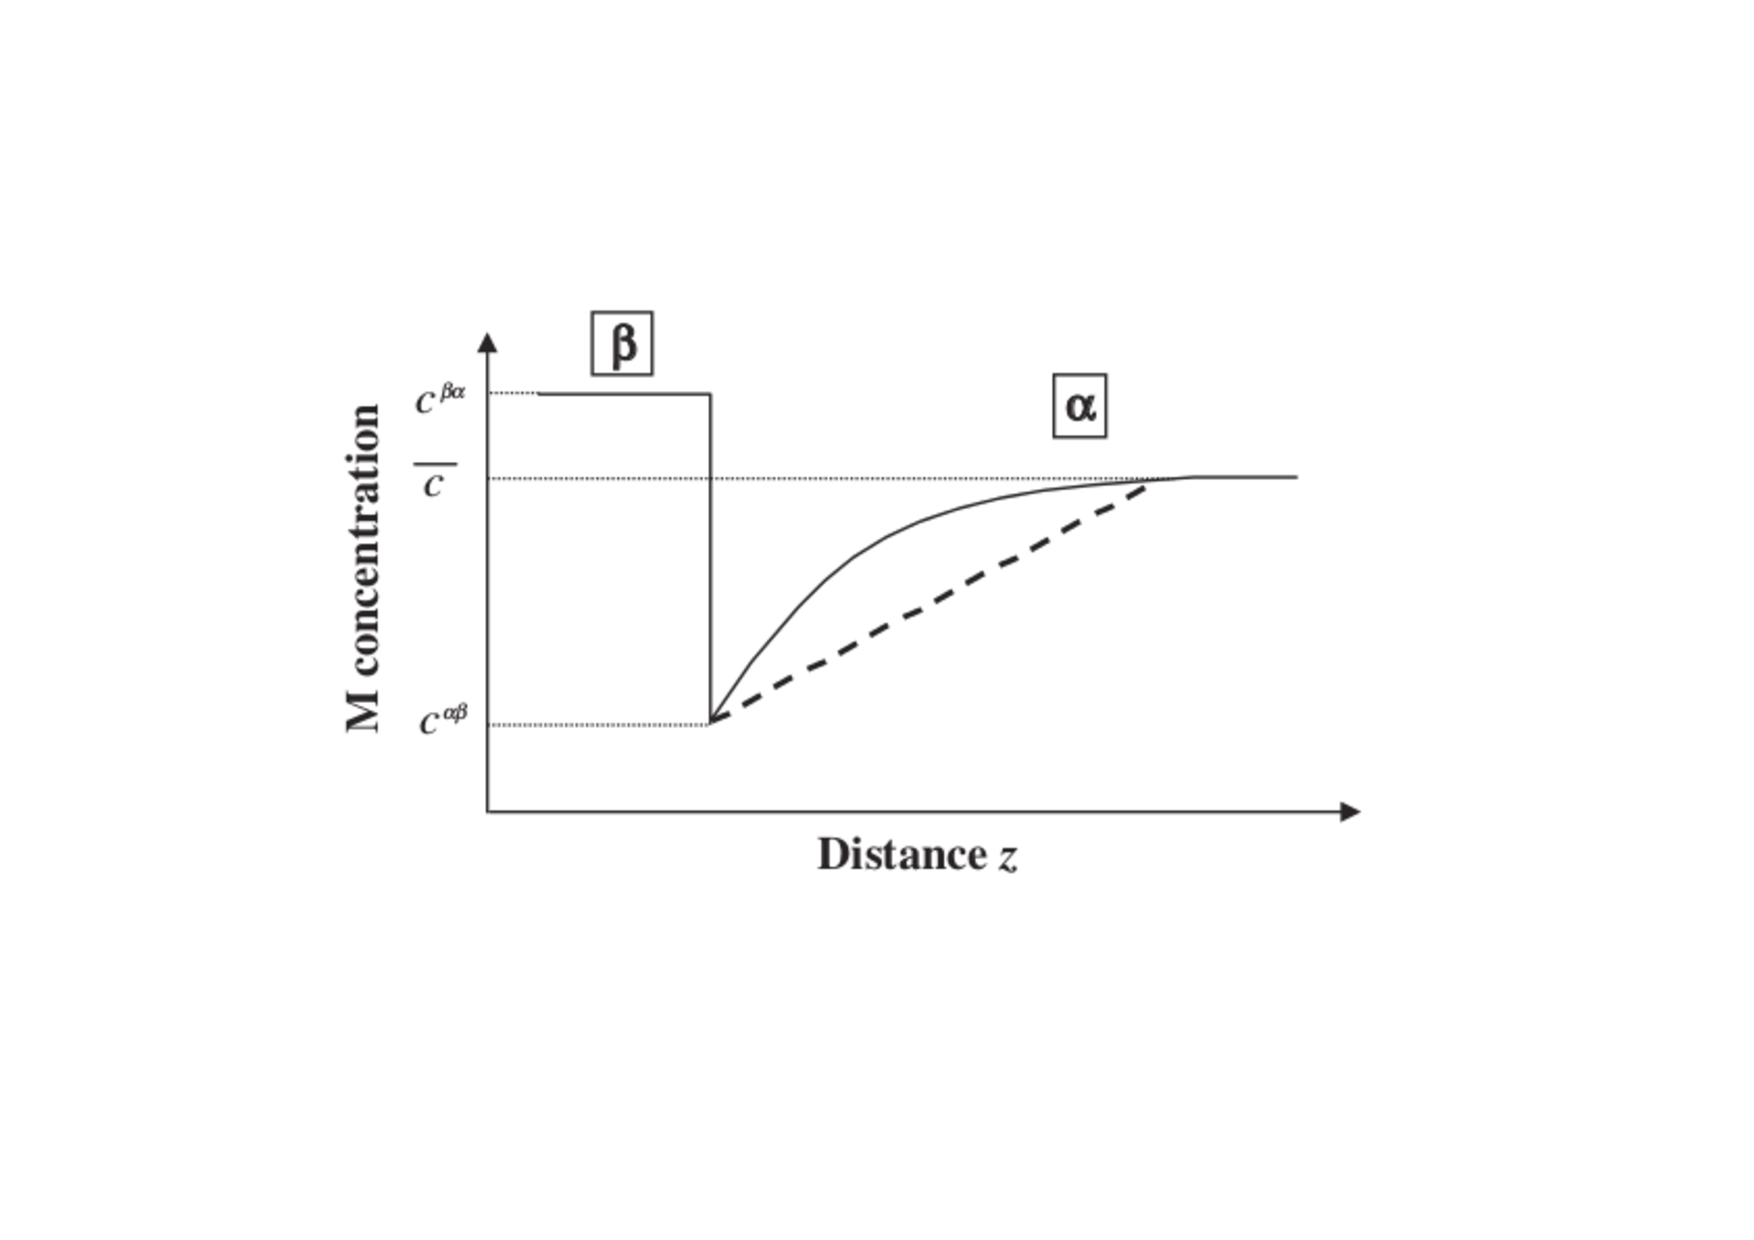
\includegraphics[width=6cm]{prec.pdf}
%\caption{Schematic showing precipitate formation in a binary alloy}
\label{fig:prec_g}
\end{figure}
\end{column}
\end{columns}
\end{frame}
%---------------------------------------
\begin{frame}
\frametitle{Growth: MC precipitate}
\begin{block}{Growth: MC governing equation}
\[
$$ $v(c_X^{\beta \alpha}-c_X^{\alpha \beta})=-D_X\nabla c_X$ $$
\]
\end{block}
\begin{columns}
\begin{column}{0.6\textwidth}
\begin{itemize}
\item C: interstitial atom $\rightarrow$ $D_C >> D_\mathrm{Nb}$. 
\item Flux of C and Nb should almost match. 
%\item a $\rightarrow$ $\bar{c_C}$ and $\bar{c_M}$ $\rightarrow$ average compositions in matrix.
\item Movement from b to c and a to c
\begin{itemize}
	\item b $\rightarrow$ initial C composition such that C gradient minimized and M gradient maximised.
	\item As solute from matrix depleted, the average composition moves from a to c.
	\item c $\rightarrow$ Equilibrium
\end{itemize}
\end{itemize}
\end{column}
\begin{column}{0.4\textwidth}
\begin{figure}
\centering
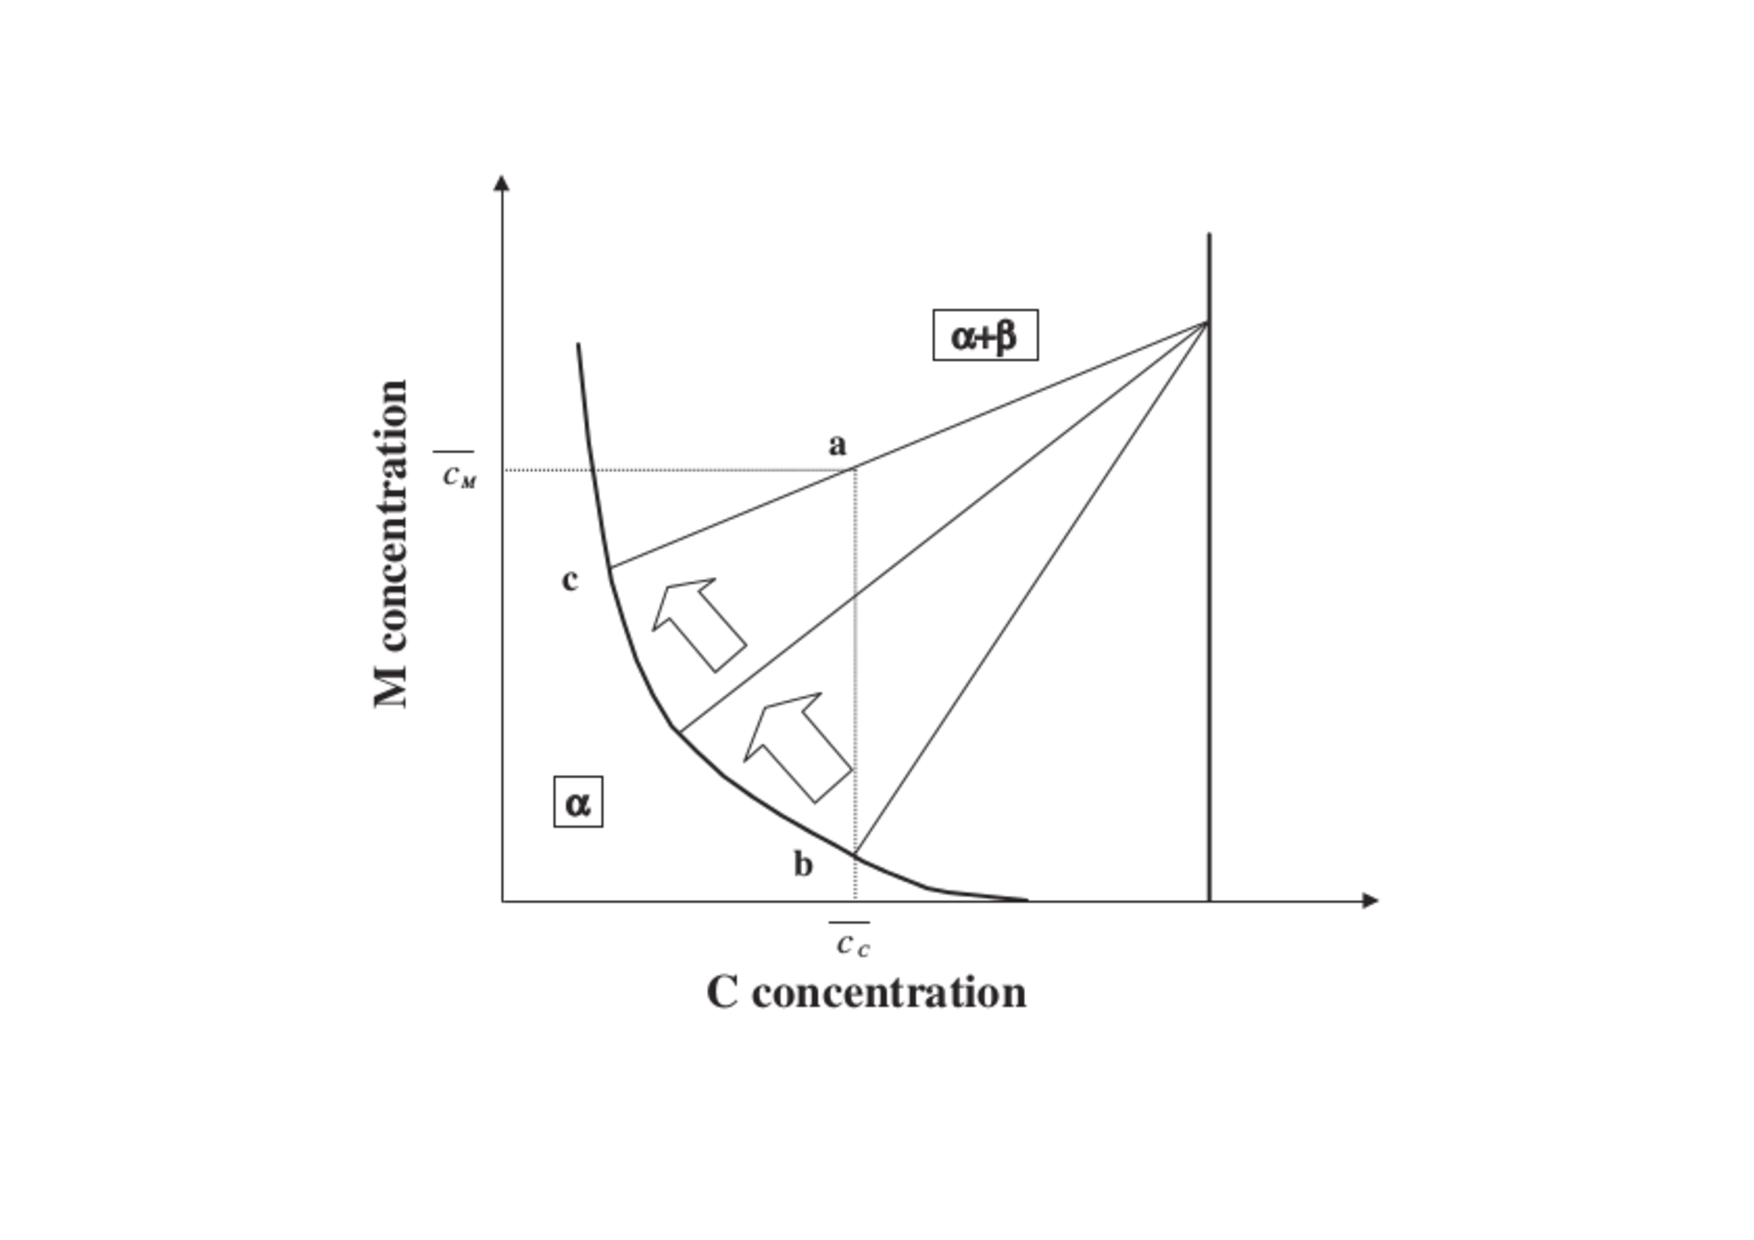
\includegraphics[width=6cm]{phd.pdf}
%\caption{Diffusion conditions in a MC precipitate and matrix system}
\label{fig:diff}
\end{figure}
\end{column}
\end{columns}
\end{frame}
%---------------------------------------
\begin{frame}
\frametitle{Capillarity}
\begin{block}{Capillarity equation}
\[
$$ $c_{r,\mathrm{M}}^{\alpha \beta}=\bigg(1+\frac{\sigma}{kT}\frac{v^\beta}{r}\frac{1-c_{\mathrm{M}}^{\alpha \beta}}{c_{\mathrm{M}}^{\beta \alpha}-c_{\mathrm{M}}^{\alpha \beta}}\bigg)c_{\mathrm{M}}^{\alpha \beta}$ $$
\]
\end{block}
%\begin{block}{Growth: solution}
%\[
%$$ $z=\alpha_3\sqrt{Dt}$ $$ 
%$$ $\alpha_3=\sqrt{2\frac{\bar{c}-c^{\alpha \beta}}{c^{\beta \alpha}-\bar{c}}}$ $$
%\]
%\end{block}
\begin{itemize}
\item Phase boundaries $\rightarrow$ modified
\item Reduces amount of small sized precipitates
\item Larger the precipitate, lower is the solute content at its interface $\rightarrow$ drives coarsening 
\end{itemize}
\end{frame}
%-----------------------------------------
\begin{frame}
\frametitle{Calculations and results}
\begin{itemize}
\item CALPHAD description and solubility products$\rightarrow$ Volume Gibbs energy
\item Fe-Nb-C system considered 
\item Parameters varied: $N_0$ and $\sigma$.
\item Close agreement with experimental data.
\item Interfacial energy 15 times stronger impact than number of nucleation sites. 
\end{itemize}
\end{frame}
%--------------------------------------------------
\begin{frame}
\frametitle{Parameters obtained}
\begin{table}
\centering
%\hspace*{-3em}
\caption{Results from modeling}
%\hspace*{-5em}
\begin{tabular}{ l c l }
\hline
 & Number density of sites: $N_0$ (m$^{-3}$&) \\
NbN & & $2\times10^{12}$ \\
Fe$_2$Nb & & $3\times10^{11}$ \\
Fe$_3$Nb$_3$C & & $3\times10^{12}$ \\
 & Interfacial energy: $\sigma$( J m$^{-2}$) & \\
NbN & &  0.230\\
Fe$_2$Nb & & 0.280 \\
Fe$_3$Nb$_3$C & & 0.330 \\
\hline
\end{tabular}
\label{tab:res}
\end{table}
\end{frame}
%------------------------------------------------
\begin{frame}
\frametitle{Volume fraction}
\begin{columns}
\begin{column}{0.5\textwidth}
\begin{itemize}
\item Precipitation sequence verified
\item Increases and saturates after some time \\ $\rightarrow$ Simultaneous dissolution of smaller particles + coarsening of the larger particles.
\end{itemize}
\end{column}
\begin{column}{0.5\textwidth}
\begin{figure}
\centering
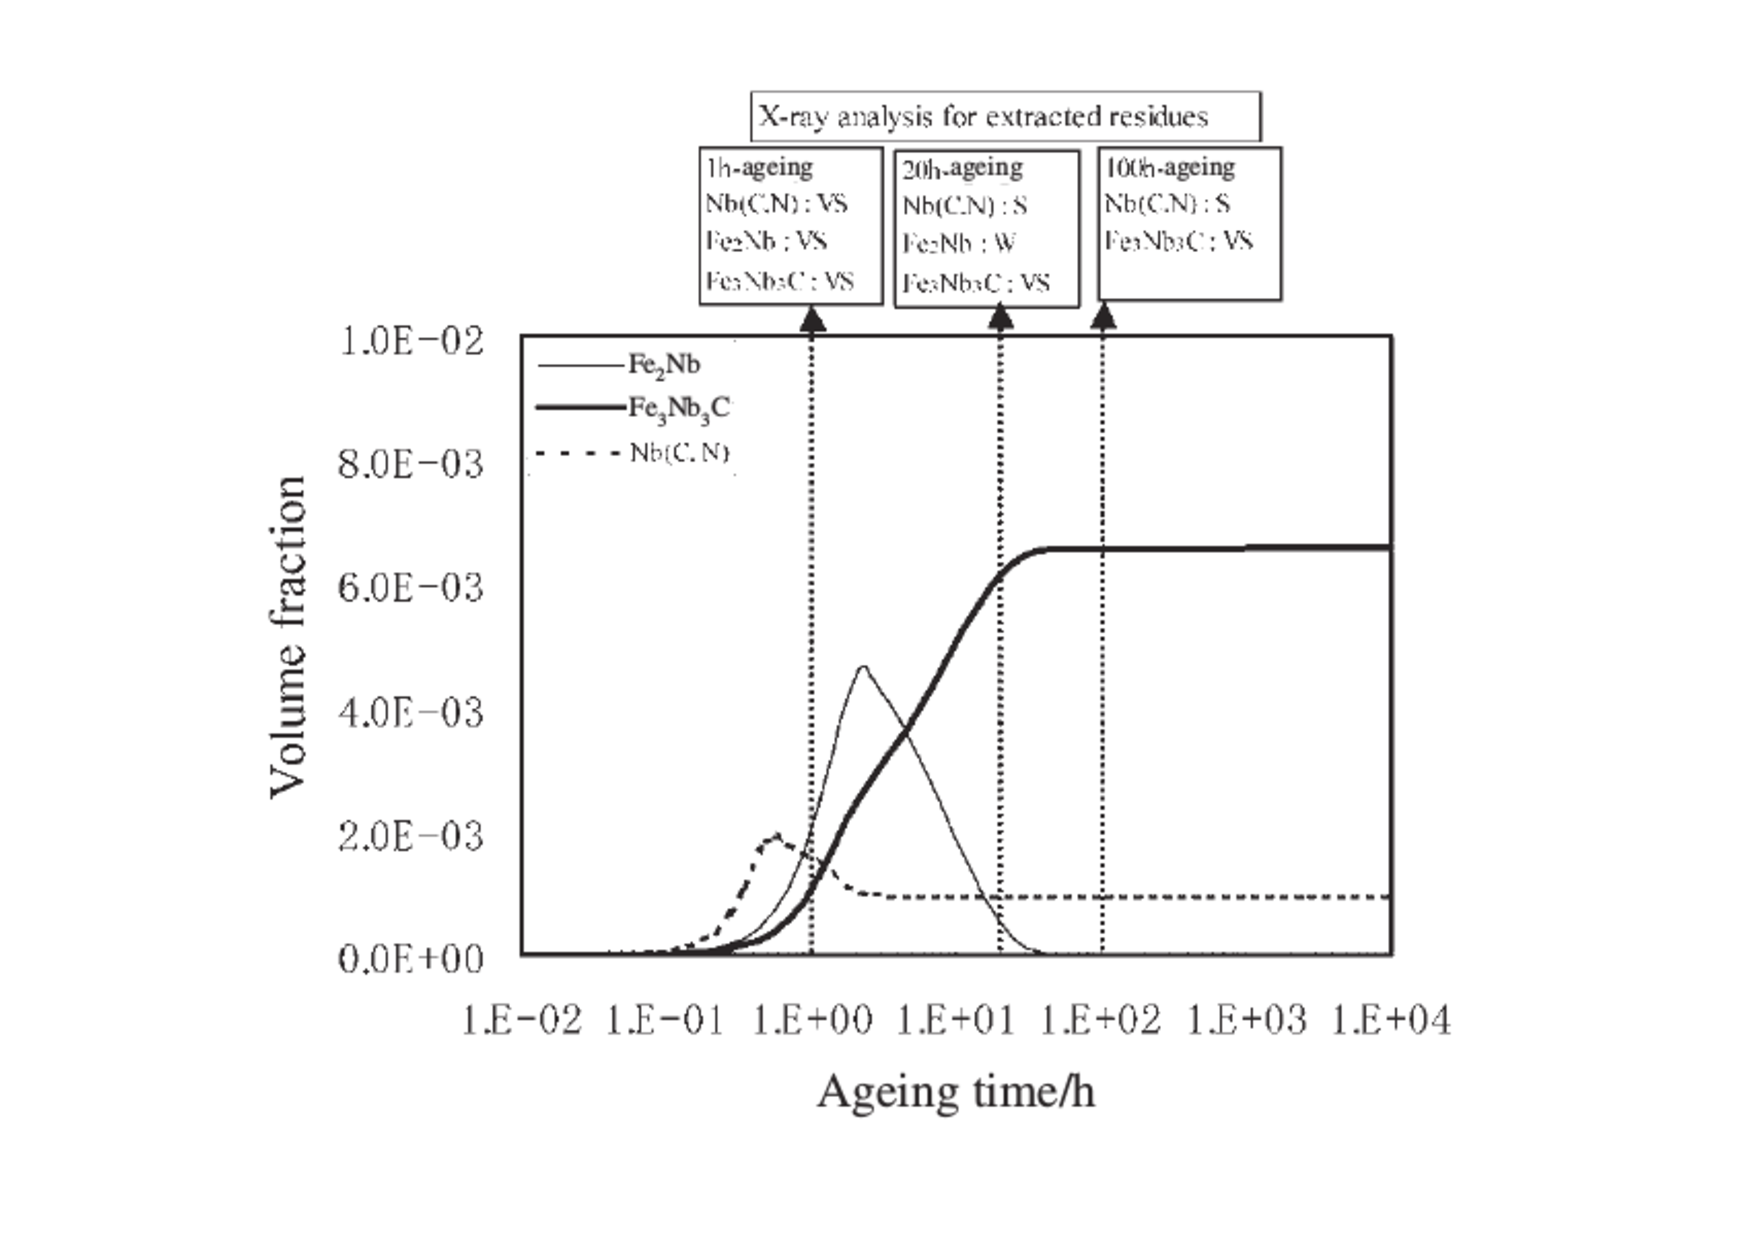
\includegraphics[width=6cm]{vol.pdf}
%\caption{Volume fraction calculated as compared to experiments}
\label{fig:vol}
\end{figure}
\end{column}
\end{columns}
\end{frame}
%---------------------------------------
\begin{frame}
\frametitle{Precipitate sizes}
\begin{columns}
\begin{column}{0.5\textwidth}
\begin{itemize}
\item Mean radius increases and stabilizes after some time 
\item Larger particle: radii increases $\rightarrow$ Coarsening
\item Smaller particle: radii decreases $\rightarrow$ Dissolution
\item The number density of precipitates, decreasing during coarsening.
\end{itemize}
\end{column}
\begin{column}{0.5\textwidth}
\begin{figure}
\centering
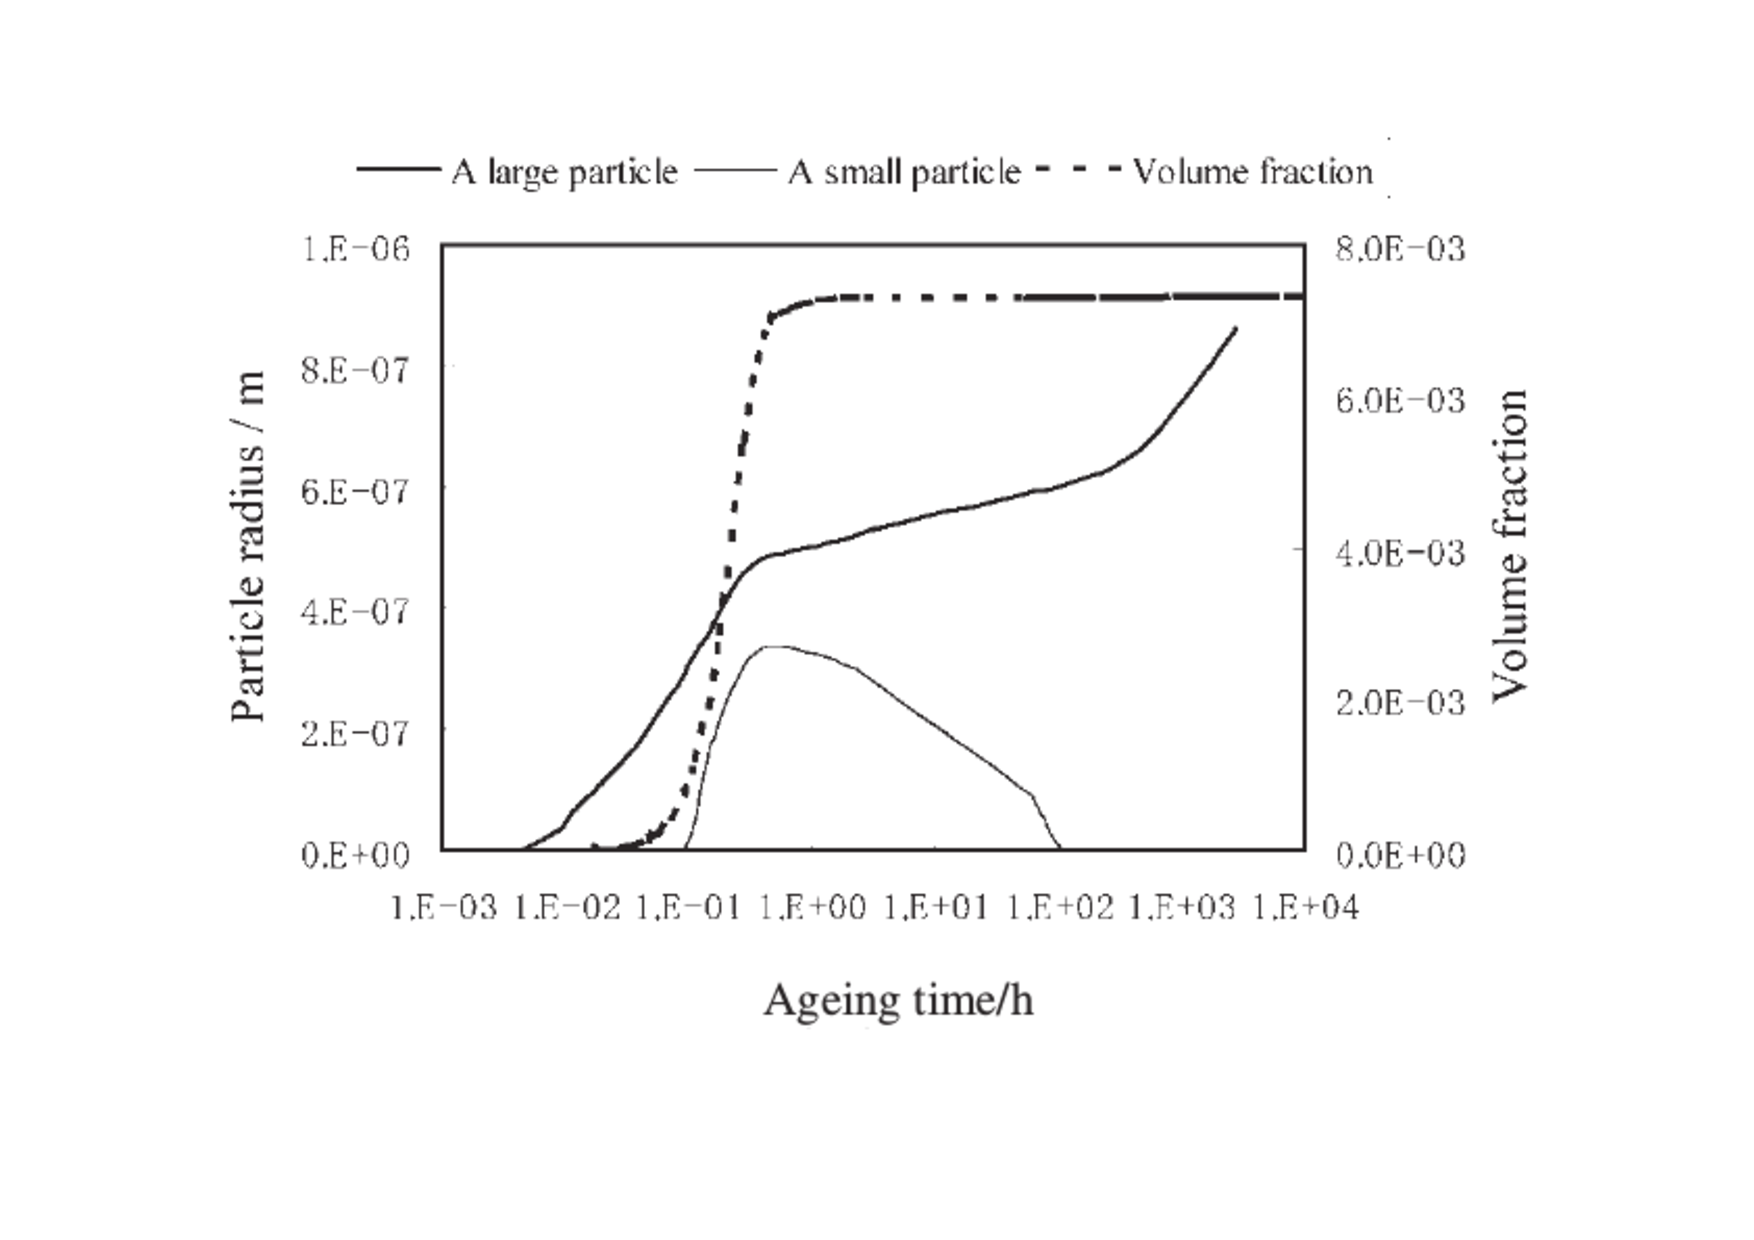
\includegraphics[width=6cm]{size.pdf}
%\caption{Precipitate sizes calculated for Fe$_3$Nb$_3$C}
\label{fig:size}
\end{figure}
\end{column}
\end{columns}
\end{frame}
%----------------------------------------------
\begin{frame}
\frametitle{Summary}
\begin{itemize}
\item Fe-Nb-C system considered 
\item Parameters varied: $N_0$ and $\sigma$.
\item Close agreement with experimental data.
\item Interfacial energy 15 times stronger impact than number of nucleation sites. 
\item Larger particle: radii increases $\rightarrow$ Coarsening
\item Smaller particle: radii decreases $\rightarrow$ Dissolution
\end{itemize}
\end{frame}
\end{document}
